% Chapter 1
\chapter{Introduction} % Main chapter title

\label{Chapter1} % For referencing the chapter elsewhere, use \ref{Chapter1} 

\lhead{Chapter 1. \emph{Introduction}} % This is for the header on each page - perhaps a shortened title

%----------------------------------------------------------------------------------------
\section{Context}
\label{context}
The rapidly progressing digital revolution have infused enormous amount of images and video, which is growing constantly. Dealing with this large scale data calls for software application for enhancing image quality is the topic of Image Processing. Although image processing algorithms are getting accurate day by day, there is constant pressure on algorithms to deal with noise. It is inherent to the acquisition tools. State of the art preprocessing and postprocessing algorithms are being developed to suppress noise with altering the important content. The noise in an image is reduced by convolving the image with a Gaussian function. The above common approach blurs significant features and destroys some of the geometric information in the image \citep{Thor2009}. Image processing task are often tackled with geometric methods, which targets to understand the geometric configuration and relation between the observed objects. Manifold learning algorithms are one such geometric methods.

\section{Manifold Learning}
Manifold learning is form of unsupervised machine learning algorithms, which  extract low-dimensional structure from high dimensional data. These algorithms typically try to unfold the underlying manifold so that Euclidean distance in the new space is a meaningful measure of distance metrics between any pair of points. Manifold learning assumes that the data lies approximately on a low dimensional surface embedded in a high dimensional space \citep{Tal2008}. It can be further illustrated  using figure \ref{fig:manifold}, where manifold learning algorithms for non-linear data builds an embedding function $f$ mapping $\mathcal{M}$ to $\mathbb{R}^2$.

\begin{figure}[ht]
\begin{center}
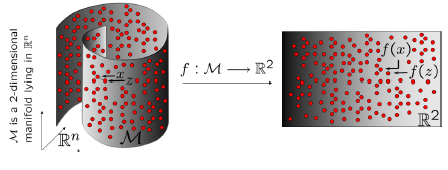
\includegraphics[width=\textwidth]{./Figures/manifold.png}
\caption{Manifold Learning \citep{Ety2008}}
\label{fig:manifold}
\end{center}
\end{figure}



\section{Motivation}
Consider the example of an image sequence. In the absence of features such as contour
points or wavelet coefficients, each image is a point in a space of dimension equal
to the number of image pixels. When facing an observation space of possibly tens or
hundreds of thousands of dimensions, it is often reasonable to assume that the data is not
dense in such a space and that many of the measured variables must be dependent with
only a few free parameters that are embedded in the observed variables, frequently in a
nonlinear way. Assuming that the number of free parameters remains the same throughout
the observations, and also assuming spatially smooth variation of the parameters,
we have geometric restrictions which can be well modeled as a manifold. Learning this manifold is a natural approach to the problem of modeling the data, with the advantage
of allowing nonlinear dimensionality reduction

\section{Contribution}
This paper presents a novel manifold learning approach for high dimensional
data, with emphasis on the problem of anomaly detection in image.

\section{Organization}




 

%----------------------------------------------------------------------------------------


